\uuid{grdy}
\exo7id{5389}
\titre{exo7 5389}
\auteur{rouget}
\organisation{exo7}
\datecreate{2010-07-06}
\isIndication{false}
\isCorrection{true}
\chapitre{Continuité, limite et étude de fonctions réelles}
\sousChapitre{Continuité : théorie}

\contenu{
\texte{
Etudier en chaque point de $\Rr$ l'existence d'une limite à droite, à gauche, la continuité de la fonction $f$ définie par $f(x)=xE(\frac{1}{x})$ si $x\neq0$ et $1$ si $x=0$.
}
\reponse{
Donnons tout d'abord une expression plus explicite de $f(x)$ pour chaque réel $x$.

Si $x>1$, alors $\frac{1}{x}\in]0,1[$ et donc, $f(x)=0$.

Si $\exists p\in\Nn^*/\;x\in]\frac{1}{p+1},\frac{1}{p}],\;f(x)=px$.

$f(0)=1$ (et plus généralement, $\forall p\in\Zz^*,\;f(\frac{1}{p})=1)$.

Si $x\leq-1$, alors $\frac{1}{x}\in[-1,0[$ et donc, $f(x)=-x$. 

Enfin, si $\exists p\in\Zz^\setminus\{-1\}$ tel que $x\in]\frac{1}{p+1},\frac{1}{p}]$, alors $\frac{1}{p+1}<x\leq\frac{1}{p}(<0)$ fournit, par décroissance de la fonction $x\mapsto\frac{1}{x}$ sur $]-\infty,0[$, $p\leq\frac{1}{x}<p+1(<0)$ et donc $f(x)=px$.

Etude en $0$. $\forall x\in\Rr^*,\;\frac{1}{x}-1<E(\frac{1}{x})\leq\frac{1}{x}$ et donc $1-x<f(x)\leq1$ si $x>0$ et $1\leq f(x)<1-x$ si $x<0$. Par suite, 

$$\forall x\in\Rr,\;|f(x)-1\leq|x|,$$

et $\lim_{x\rightarrow 0}f(x)=1$. $f$ est donc continue en $0$.

$f$ est affine sur chaque intervalle de la forme $]\frac{1}{p+1},\frac{1}{p}]$ pour $p$ élément de $\Zz\setminus\{-1,0\}$ et donc est continue sur ces intervalles et en particulier continue à gauche en chaque $\frac{1}{p}$. $f$ est affine sur $]-\infty,-1]$ et aussi sur $]1,+\infty[$ et est donc continue sur ces intervalles. Il reste donc à analyser la continuité à droite en $\frac{1}{p}$, pour $p$ entier relatif non nul donné. Mais,

$$f(\frac{1}{p}^+)=\lim_{x \rightarrow\frac{1}{p},\;x>\frac{1}{p}}(x(p-1))=1-\frac{1}{p}\neq 1=f(\frac{1}{p}).$$

$f$ est donc discontinue à droite en tout $\frac{1}{p}$ où $p$ est un entier relatif non nul donné.

Graphe de $f$~:

$$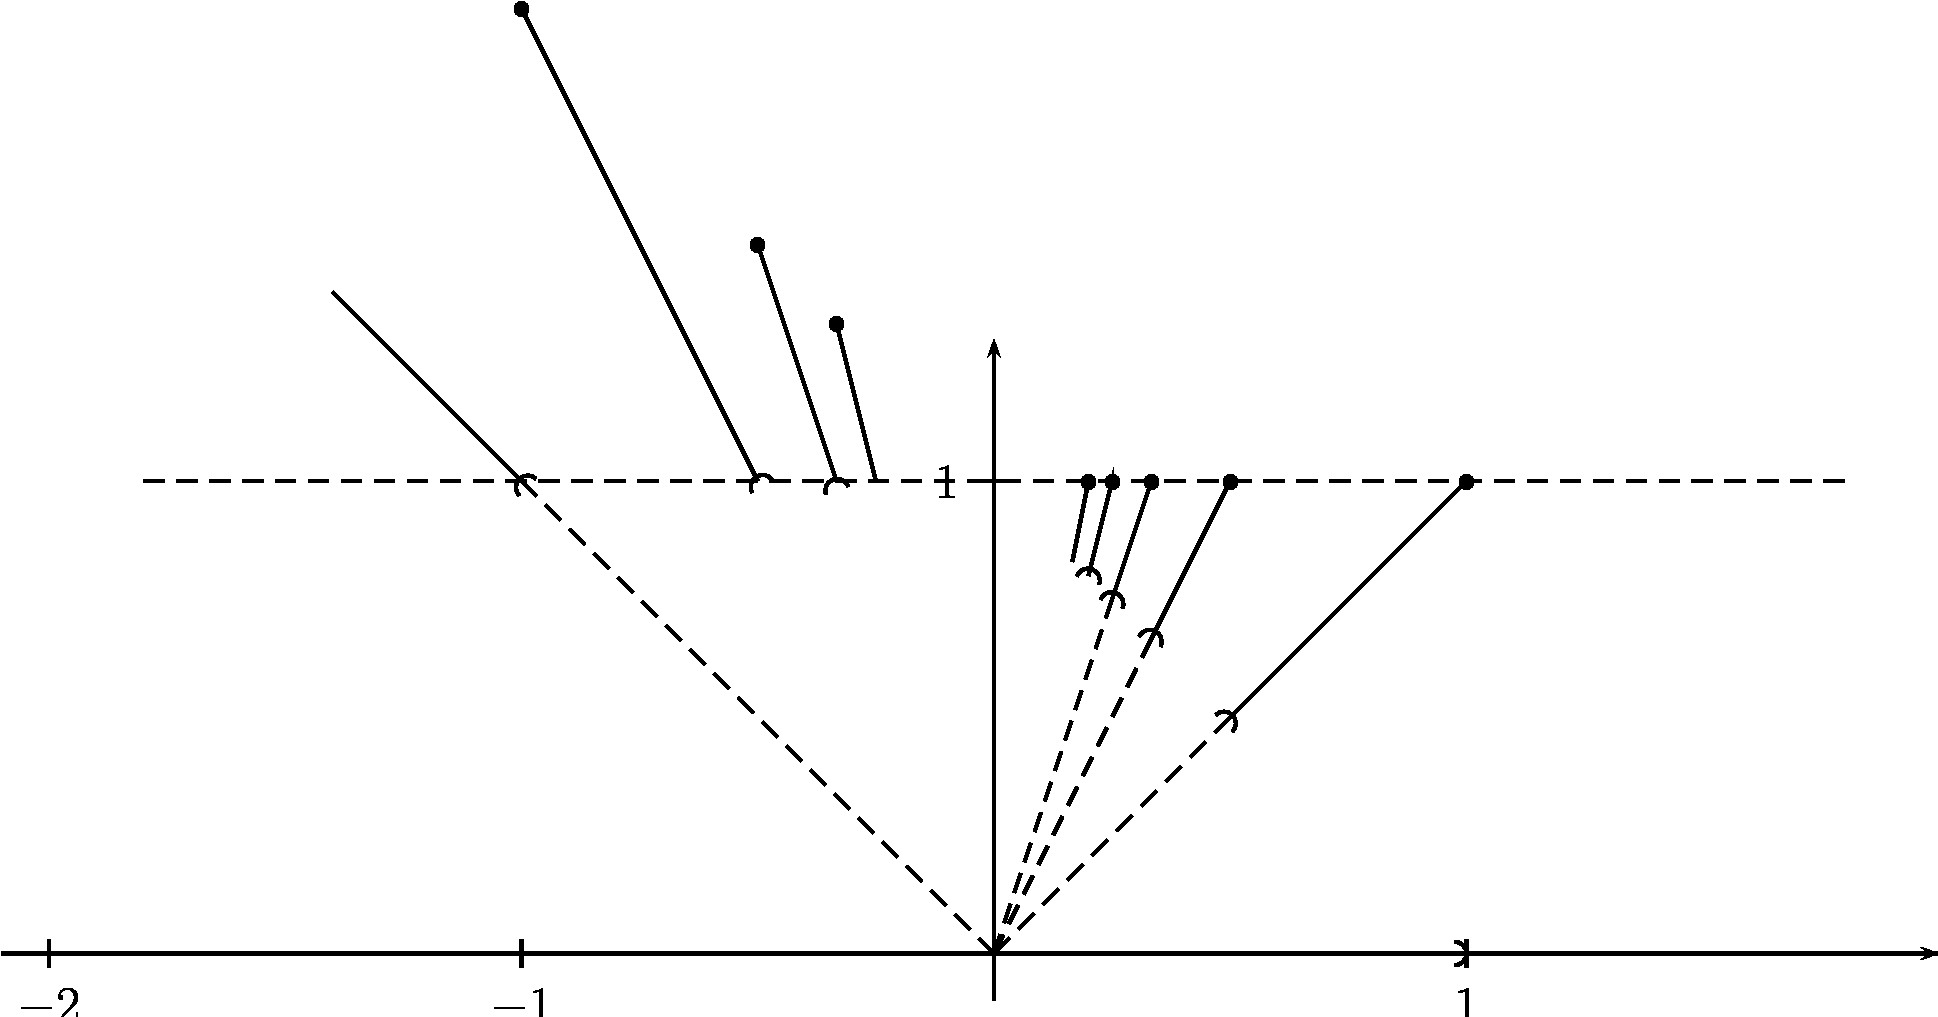
\includegraphics{../images/img005389-1}$$
}
}
